%% fig_extprofile.tex   (generated by make_frontier.py; do not edit by hand)
%% Lower bounds for the self-Ext of an object with the Chern character of an exceptional class, and the Euler characteristic balance.
\documentclass[tikz,border=8pt]{standalone}
\usepackage{amsmath,amssymb}
\usetikzlibrary{arrows.meta,calc,decorations.pathreplacing}
%% palette.tex -- shared colour definitions for the figures
\definecolor{PInk}{RGB}{26,32,44}
\definecolor{PBlue}{RGB}{37,82,139}
\definecolor{PTeal}{RGB}{23,127,125}
\definecolor{POchre}{RGB}{193,138,44}
\definecolor{PClay}{RGB}{178,74,58}
\definecolor{PSlate}{RGB}{108,122,137}
\definecolor{PViolet}{RGB}{110,86,150}
\definecolor{WBlue}{RGB}{223,234,246}
\definecolor{WTeal}{RGB}{220,238,236}
\definecolor{WOchre}{RGB}{250,240,218}
\definecolor{WClay}{RGB}{247,229,224}
\definecolor{WSlate}{RGB}{238,241,244}
\definecolor{PMag}{RGB}{158,58,110}
\definecolor{PGrass}{RGB}{62,124,66}
\definecolor{PAmber}{RGB}{214,112,38}
\definecolor{PIndigo}{RGB}{58,64,140}
\definecolor{PRule}{RGB}{176,186,197}

%% shared macros so the standalone figures match the paper
\providecommand{\QQ}{\mathbb{Q}}
\providecommand{\ZZ}{\mathbb{Z}}
\providecommand{\RR}{\mathbb{R}}
\providecommand{\CC}{\mathbb{C}}
\providecommand{\PP}{\mathbb{P}}
\providecommand{\Kx}{K^{\times}}
\providecommand{\HW}{W}
\providecommand{\Nm}{\mathrm{N}}
\providecommand{\Hdg}{\mathrm{Hdg}}
\providecommand{\NS}{\mathrm{NS}}
\providecommand{\cA}{\mathcal{A}}
\providecommand{\cD}{\mathcal{D}}
\providecommand{\cF}{\mathcal{F}}
\providecommand{\cP}{\mathcal{P}}
\providecommand{\cO}{\mathcal{O}}
\providecommand{\cQ}{\mathcal{Q}}
\providecommand{\bbar}[1]{\overline{#1}}
\providecommand{\ch}{\operatorname{ch}}
\providecommand{\End}{\mathrm{End}}

\newcommand{\hcimp}{\,\textcolor{PIndigo}{\tiny$\Leftarrow\mathbf{HC}$}}
\begin{document}
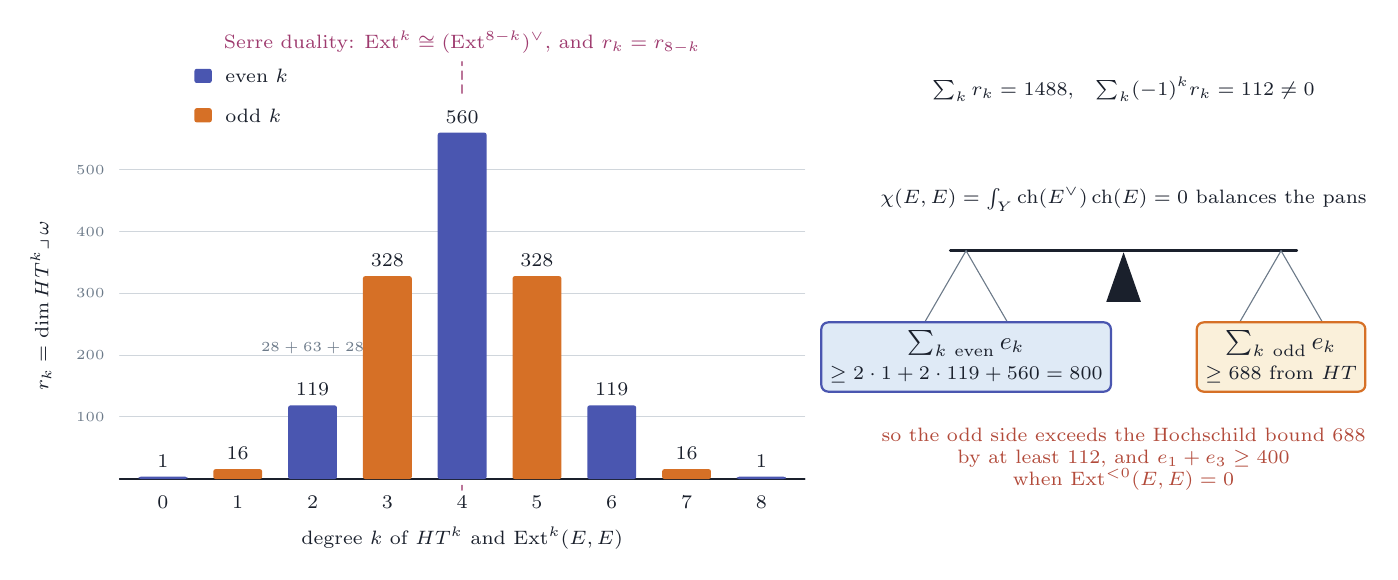
\begin{tikzpicture}[x=1cm,y=1cm,line join=round,line cap=round,
  font=\small,text=PInk]
  \definecolor{BEven}{HTML}{4A56B0}
  \definecolor{BOdd}{HTML}{D67026}
  \draw[PRule!60,line width=0.30pt] (-0.55,0.79) -- (8.15,0.79);
  \node[text=PSlate,inner sep=1pt,align=center,font=\tiny,anchor=east] at (-0.70,0.79) {$100$};
  \draw[PRule!60,line width=0.30pt] (-0.55,1.57) -- (8.15,1.57);
  \node[text=PSlate,inner sep=1pt,align=center,font=\tiny,anchor=east] at (-0.70,1.57) {$200$};
  \draw[PRule!60,line width=0.30pt] (-0.55,2.36) -- (8.15,2.36);
  \node[text=PSlate,inner sep=1pt,align=center,font=\tiny,anchor=east] at (-0.70,2.36) {$300$};
  \draw[PRule!60,line width=0.30pt] (-0.55,3.14) -- (8.15,3.14);
  \node[text=PSlate,inner sep=1pt,align=center,font=\tiny,anchor=east] at (-0.70,3.14) {$400$};
  \draw[PRule!60,line width=0.30pt] (-0.55,3.93) -- (8.15,3.93);
  \node[text=PSlate,inner sep=1pt,align=center,font=\tiny,anchor=east] at (-0.70,3.93) {$500$};
  \draw[PInk,line width=0.60pt] (-0.55,0.00) -- (8.15,0.00);
  \draw[PMag!70,line width=0.50pt,dash pattern=on 3pt off 2pt] (3.80,4.90) -- (3.80,5.30);
  \draw[PMag!70,line width=0.50pt] (3.80,-0.08) -- (3.80,-0.14);
  \node[text=PMag,inner sep=1pt,align=center,font=\scriptsize] at (3.80,5.55) {Serre duality: $\mathrm{Ext}^{k}\cong(\mathrm{Ext}^{8-k})^{\vee}$, and $r_{k}=r_{8-k}$};
  \fill[BEven,rounded corners=0.8pt] (-0.310,0) rectangle (0.310,0.030);
  \node[text=PInk,inner sep=1pt,align=center,font=\scriptsize] at (0.00,0.23) {$1$};
  \node[text=PInk,inner sep=1pt,align=center,font=\scriptsize] at (0.00,-0.30) {$0$};
  \fill[BOdd,rounded corners=0.8pt] (0.640,0) rectangle (1.260,0.126);
  \node[text=PInk,inner sep=1pt,align=center,font=\scriptsize] at (0.95,0.33) {$16$};
  \node[text=PInk,inner sep=1pt,align=center,font=\scriptsize] at (0.95,-0.30) {$1$};
  \fill[BEven,rounded corners=0.8pt] (1.590,0) rectangle (2.210,0.935);
  \node[text=PInk,inner sep=1pt,align=center,font=\scriptsize] at (1.90,1.14) {$119$};
  \node[text=PInk,inner sep=1pt,align=center,font=\scriptsize] at (1.90,-0.30) {$2$};
  \fill[BOdd,rounded corners=0.8pt] (2.540,0) rectangle (3.160,2.577);
  \node[text=PInk,inner sep=1pt,align=center,font=\scriptsize] at (2.85,2.78) {$328$};
  \node[text=PInk,inner sep=1pt,align=center,font=\scriptsize] at (2.85,-0.30) {$3$};
  \fill[BEven,rounded corners=0.8pt] (3.490,0) rectangle (4.110,4.400);
  \node[text=PInk,inner sep=1pt,align=center,font=\scriptsize] at (3.80,4.60) {$560$};
  \node[text=PInk,inner sep=1pt,align=center,font=\scriptsize] at (3.80,-0.30) {$4$};
  \fill[BOdd,rounded corners=0.8pt] (4.440,0) rectangle (5.060,2.577);
  \node[text=PInk,inner sep=1pt,align=center,font=\scriptsize] at (4.75,2.78) {$328$};
  \node[text=PInk,inner sep=1pt,align=center,font=\scriptsize] at (4.75,-0.30) {$5$};
  \fill[BEven,rounded corners=0.8pt] (5.390,0) rectangle (6.010,0.935);
  \node[text=PInk,inner sep=1pt,align=center,font=\scriptsize] at (5.70,1.14) {$119$};
  \node[text=PInk,inner sep=1pt,align=center,font=\scriptsize] at (5.70,-0.30) {$6$};
  \fill[BOdd,rounded corners=0.8pt] (6.340,0) rectangle (6.960,0.126);
  \node[text=PInk,inner sep=1pt,align=center,font=\scriptsize] at (6.65,0.33) {$16$};
  \node[text=PInk,inner sep=1pt,align=center,font=\scriptsize] at (6.65,-0.30) {$7$};
  \fill[BEven,rounded corners=0.8pt] (7.290,0) rectangle (7.910,0.030);
  \node[text=PInk,inner sep=1pt,align=center,font=\scriptsize] at (7.60,0.23) {$1$};
  \node[text=PInk,inner sep=1pt,align=center,font=\scriptsize] at (7.60,-0.30) {$8$};
  \node[text=PInk,inner sep=1pt,align=center,font=\scriptsize] at (3.80,-0.75) {degree $k$ of $HT^{k}$ and $\mathrm{Ext}^{k}(E,E)$};
  \node[text=PInk,inner sep=1pt,align=center,font=\scriptsize,rotate=90] at (-1.55,2.20) {$r_{k}=\dim HT^{k}\lrcorner\,\omega$};
  \node[text=PSlate,inner sep=1pt,align=center,font=\tiny] at (1.90,1.66) {$28+63+28$};
  \fill[BEven,rounded corners=0.8pt] (0.40,5.03) rectangle (0.62,5.21);
  \node[text=PInk,inner sep=1pt,align=center,font=\scriptsize,anchor=west] at (0.75,5.12) {even $k$};
  \fill[BOdd,rounded corners=0.8pt] (0.40,4.53) rectangle (0.62,4.71);
  \node[text=PInk,inner sep=1pt,align=center,font=\scriptsize,anchor=west] at (0.75,4.62) {odd $k$};
  \draw[PInk,line width=1.00pt] (10.00,2.90) -- (14.40,2.90);
  \fill[PInk] (11.98,2.25) -- (12.42,2.25) -- (12.20,2.88) -- cycle;
  \draw[PSlate,line width=0.40pt] (10.20,2.90) -- (9.65,1.95);
  \draw[PSlate,line width=0.40pt] (10.20,2.90) -- (10.75,1.95);
  \draw[PSlate,line width=0.40pt] (14.20,2.90) -- (13.65,1.95);
  \draw[PSlate,line width=0.40pt] (14.20,2.90) -- (14.75,1.95);
  \node[draw=BEven,fill=WBlue,rounded corners=2.5pt,inner sep=3pt,line width=0.80pt,align=center] at (10.20,1.55) {$\sum_{k\ \mathrm{even}}e_{k}$\\{\scriptsize$\ge2\cdot1+2\cdot119+560=800$}};
  \node[draw=BOdd,fill=WOchre,rounded corners=2.5pt,inner sep=3pt,line width=0.80pt,align=center] at (14.20,1.55) {$\sum_{k\ \mathrm{odd}}e_{k}$\\{\scriptsize$\ge688$ from $HT$}};
  \node[text=PInk,inner sep=1pt,align=center,font=\scriptsize] at (12.20,3.55) {$\chi(E,E)=\int_{Y}\ch(E^{\vee})\ch(E)=0$ balances the pans};
  \node[text=PClay,inner sep=1pt,align=center,font=\scriptsize] at (12.20,0.25) {so the odd side exceeds the Hochschild bound $688$\\by at least $112$, and $e_{1}+e_{3}\ge400$\\when $\mathrm{Ext}^{<0}(E,E)=0$};
  \node[text=PInk,inner sep=1pt,align=center,font=\scriptsize] at (12.20,4.95) {$\sum_{k}r_{k}=1488$,\quad $\sum_{k}(-1)^{k}r_{k}=112\neq0$};
\end{tikzpicture}
\end{document}
